\documentclass[12pt,
               a4paper,
               article,
               oneside,
               oldfontcommands,
               UKenglish]{memoir}


\usepackage[utf8]{inputenc}
\usepackage[T1]{fontenc}
\usepackage{lmodern}
\usepackage[scaled]{beramono}
\usepackage[final]{microtype}
\usepackage{amssymb}
\usepackage{mathtools}
\usepackage{amsthm}
\usepackage{thmtools}
\usepackage{babel}
\usepackage{csquotes}
\usepackage[nodayofweek]{datetime}
\usepackage{listings}
\lstset{basicstyle = \ttfamily}
\usepackage{textcomp}
\usepackage{siunitx}
\usepackage{xcolor}
\usepackage{graphicx}
\usepackage[colorlinks, allcolors = uiolink]{hyperref}


\usepackage{tikz}
\usetikzlibrary{
  graphs,
  graphs.standard
}
\renewcommand*{\chaptitlefont}{\Large\bfseries\sffamily\raggedright}
\setsecheadstyle{\large\bfseries\sffamily\raggedright}
\setsubsecheadstyle{\large\bfseries\sffamily\raggedright}
\setsubsubsecheadstyle{\normalsize\bfseries\sffamily\raggedright}
\setparaheadstyle{\normalsize\bfseries\sffamily\raggedright}
\setsubparaheadstyle{\normalsize\bfseries\sffamily\raggedright}
\setbeforesubsubsecskip{2ex}
\setaftersubsubsecskip{1ex}


\pretolerance = 2000
\tolerance    = 6000
\hbadness     = 6000


\renewcommand{\sfdefault}{phv}
\definecolor{uiolink}{HTML}{0B5A9D}


\declaretheorem[style = definition]{problem}
\declaretheorem[style = definition, sibling = problem]{exercise}


\begin{document}


\begin{titlingpage}
    \vspace*{-8em}
    \setlength{\parskip}{1.5ex plus 0.5ex minus 0.2ex}
    \setlength{\parindent}{0pt}

    \begin{flushright}
        \small\today
    \end{flushright}

    \begin{center}
        \vspace{2em}
        {
            \bfseries\sffamily\huge
            MAT2250
             \textthreequartersemdash\ Discrete Math
        }
        \vskip0.2ex
        \Large
        Mandatory assignment 1 of 1
        \vskip1ex
    \end{center}

    \subsubsection*{Submission deadline}
    Thursday 8\textsuperscript{th} April  \the\year, 14:30 in Canvas
    (\href{https://canvas.uio.no}{\underline{canvas.uio.no}}).

    \subsubsection*{Instructions}
    You can choose between scanning handwritten notes or typing the solution directly on a computer (for instance with \LaTeX).
    The assignment must be submitted as a single PDF file.
    Scanned pages must be clearly legible.
    The submission must contain your name, course and assignment number.

    It is expected that you give a clear presentation with all necessary explanations.
    Remember to include all relevant plots and figures.
    Students who fail the assignment, but have made a genuine effort at solving the exercises, are given a second attempt at revising their answers.
    All aids, including collaboration, are allowed, but the submission must be written by you and reflect your understanding of the subject.
    If we doubt that you have understood the content you have handed in, we may request that you give an oral account.

    In exercises where you are asked to write a computer program, you need to hand in the code along with the rest of the assignment.
    It is important that the submitted program contains a trial run, so that it is easy to see the result of the code.

    \subsubsection*{Application for postponed delivery}
    If you need to apply for a postponement of the submission deadline due to illness or other reasons, you have to contact the Student Administration at the Department of Mathematics (e-mail: \href{mailto:studieinfo@math.uio.no}{studieinfo@math.uio.no}) well before the deadline.

    All mandatory assignments in this course must be approved in the same semester, before you are allowed to take the final examination.

    \subsubsection*{Complete guidelines about delivery of mandatory assignments:}
    \unskip
    \begin{center}
        \unskip
        \href{http://www.uio.no/english/studies/admin/compulsory-activities/mn-math-mandatory.html}
        {
            \resizebox{\textwidth}{!}
            {\underline{uio.no/english/studies/admin/compulsory-activities/mn-math-mandatory.html}}
        }
        \vspace{1ex}
        \vfill
        GOOD LUCK!
    \end{center}
\end{titlingpage}
week-11/

\noindent
{\bf
You are highly encouraged to collaborate with other students on the problem set.  If you need help connecting with others in the course, let me know by email.
You must include the names of any students who you collaborated with. Remember: the write up of all solutions must be your own! }
%% Correct typesetting of percentages: \SI{60}{\percent}


\noindent


\begin{problem}
{\bf Stirling numbers of the 2nd kind and generating functions}

\begin{enumerate}
\item Use a counting argument to show that  the Stirling numbers of the second kind satisfy $S_{n, 2} = 2^{n-1} -1$ for $n\geq 1$ (recall  that $S_{0, k} = 0$). Express the generating function

$$\mathcal{S}_2(z) = \sum_{n = 0}^\infty S_{n, 2} z^n$$

as a rational function.

\item Use the recurrence relation $S_{n, k} = S_{n-1, k-1} + k S_{n-1, k}$  and the formula found above for
$\mathcal{S}_2(z) $ to
prove that $$\mathcal{S}_3(z) := \sum_{n = 0}^\infty S_{n, 3} z^n =  \frac{z^3}{(1-z)(1-2z)(1-3z)}.$$

\item Use a partial fraction decomposition of the generating function $\mathcal{S}_3(z) $ to obtain a closed formula for $S_{n, 3}$.
\end{enumerate}



\end{problem}


\begin{problem}{\bf Graphs from sets}

\begin{enumerate}
%\ \\

\item Recall the hypercube graph is $Q_n = (V(Q_n), E(Q_n))$ where
$$V(Q_n) = \{ u_1 \dots u_n \ | \ u_i = 0, 1 \}$$
and
$$E(Q_n) = \{ uv \ | \ u, v \text{ binary words differing in exactly one letter} \}.$$
What are the sizes of $V(Q_n)$ and $E(Q_n)$?

\item Assuming all edges have weight 1, what is the distance in $Q_n$ from $00\dots00$ to $u = u_1u_2 \dots u_n$ ?
What is the distance in $Q_n$ between two arbitrary words $u$ and $v$?

\item Orient the edge $k = uv$  of $Q_n$ so that  $u = k^-$ and $v = k^+$ if the word $v$ contains more $1$'s  than $u$.
Prove that the orientation is acyclic. Which word corresponds to a sink and which word is a source?


\end{enumerate}


\end{problem}

\begin{problem}
{\bf Greedy algorithms}

Consider the graph $G$ with weight function prescribed along its edges:


 \begin{center}\newcommand\size{3}% distance of nodes from center

\begin{tikzpicture}

\draw [thick,black] (0,0)-- (18:\size)  node [above, midway] {3};
\draw [thick,black] (0,0)-- (90:\size)  node [left, midway] {2};
\draw [thick,black] (0,0)-- (162:\size)  node [above, midway] {1};
\draw [thick,black] (0,0)-- (234:\size)  node [above, midway] {1};
\draw [thick,black] (0,0)-- (306:\size)  node [above, midway] {3};


  \draw[thick,black]  (18:\size)--(90:\size) node [above, midway] {4};
    \draw[thick,black]  (90:\size)--(162:\size) node [above, midway] {2};
    \draw[thick,black]  (162:\size)--(234:\size) node [left, midway] {3};
    \draw[thick,black]  (234:\size)--(306:\size) node [above, midway] {2};
     \draw[thick,black]  (18:\size)--(306:\size) node [right, midway] {4};

      \node[black,circle,draw, fill= white, inner sep=2pt] at (18:\size){$u_1$};
  \node[black,circle,draw, fill= white, inner sep=2pt] at (90:\size){$u_0$};
   \node[black,circle,draw, fill= white, inner sep=2pt]at (162:\size){$u_4$};
      \node[black,circle,draw, fill= white, inner sep=2pt] at (234:\size){$u_3$};
       \node[black,circle,draw, fill= white, inner sep=2pt] at (306:\size){$u_2$};
         \node[black,circle,draw, fill= white, inner sep=2pt] at (0:0){$u_5$};
 \end{tikzpicture}
 \end{center}

\begin{enumerate}

\item Run Dijkstra's algorithm from starting vertex  $u_0$ to find a tree containing all minimal weight paths from $u_0$ with the prescribed weight function.
Write down which edge and vertex is selected at each step of the algorithm.

What is the length of the shortest weighted path in $G$ from $u_0$ to $u_3$?


\item Run Kruskal's algorithm to find a minimal spanning tree of $G$ for the given weight function.

What is the weight of a  minimal spanning tree in $G$?
Is there a unique minimal spanning tree in $G$ with this weight function?

\item Show that if the greedy algorithm on matroids from Theorem 7.13  can select two distinct bases  $B_1$ and  $B_2$ of minimal weight, then there must exist
$s_1 \in B_1$ and $s_2 \in B_2$ such that $w(s_1) = w(s_2)$.
Conclude that if the weight function $w : S \to \mathbb{R}$  is an injective  map then the greedy algorithm selects a unique minimal basis of a matroid.

Find an example of a weighted graph which shows that the converse to the above statement is false. Namely that there is a graph $G$ with weight function  $w : E \to \mathbb{R}$  which is not injective but the greedy algorithm still selects a unique minimal spanning tree.


\end{enumerate}

\end{problem}
\newpage

\begin{problem}{\bf{Matchings}}
\begin{enumerate}
\item
Consider the bipartite graph:


\begin{center}
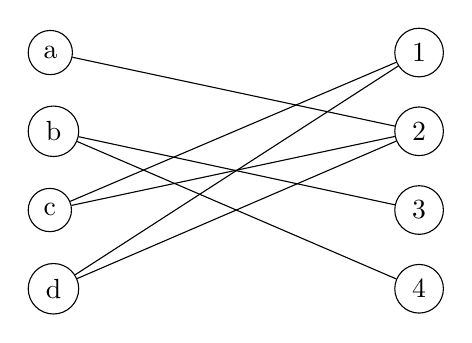
\begin{tikzpicture}
   \graph[nodes={draw, circle}, radius=.25cm,
           branch down=1 cm,       grow right sep=4cm]
           {subgraph I_nm [V={a, b, c, d}, W={1,...,4}];
  a -- { 2};
  b -- { 3, 4 };
  c -- { 1,2 };
  d -- { 1,2}
};
\end{tikzpicture}
\end{center}
Determine the matching number of $G$ and find a maximal matching.


\item The hypercube graph  $Q_n$ is bipartite, with the two disjoint vertex sets being determined by the binary  words containing an even or odd number of $1$'s.
The matching number of $Q_n$ is $2^{n-1}$. Describe a maximal matching of $Q_n$.


 \item
Let  $S$ be the set of binary words of length $n$ with $k$ number of $1's$ and let $T$ be the set of binary words of length $n$ with $k+1$ number of  $1$'s.
Let $E = \{st \ | \ s, t \text{ differ in exactly one letter}  \}$ and set  $H = (S \cup T, E)$ (notice $H$ is an induced subgraph of $Q_n$).

\begin{itemize}
\item What are  the degrees in $H$  of vertices in $S$ and vertices in $T$?

\item Prove that for any subset $A$ of $S$  we have $(k+1) |N(A)|  \geq (n-k)  |A|.$

Hint: consider the set of edges incident to $A$ and the set of edges incident to $N(A)$.

\item Use Hall's matching condition to conclude that $m(H) = |S| $ for  $k <n/2$.
\end{itemize}


Conclude that there exists an injective map $f$ from the subsets of size $k$ of $\{1, \dots, n\}$ to the subsets of size $k+1$ of $\{1, \dots ,n\}$
satisfying $I \subset f(I)$ for $k < n/2$.


\end{enumerate}


\end{problem}




\end{document}
